% DPF 09 talk on strangeness in nucleon

\documentclass[10pt]{beamer}
\usepackage{amsmath}
\usepackage{mathtools}
%\documentclass[12pt]{beamerthemeSam.sty}
\usepackage{epsf}
%\usepackage{pstricks}
%\usepackage[orientation=portrait,size=A4]{beamerposter}
\geometry{paperwidth=160mm,paperheight=120mm}
%DT favorite definitions
\def\LL{\left\langle}	% left angle bracket
\def\RR{\right\rangle}	% right angle bracket
\def\LP{\left(}		% left parenthesis
\def\RP{\right)}	% right parenthesis
\def\LB{\left\{}	% left curly bracket
\def\RB{\right\}}	% right curly bracket
\def\PAR#1#2{ {{\partial #1}\over{\partial #2}} }
\def\PARTWO#1#2{ {{\partial^2 #1}\over{\partial #2}^2} }
\def\PARTWOMIX#1#2#3{ {{\partial^2 #1}\over{\partial #2 \partial #3}} }

\def\rightpartial{{\overrightarrow\partial}}
\def\leftpartial{{\overleftarrow\partial}}
\def\diffpartial{\buildrel\leftrightarrow\over\partial}

\def\BI{\begin{itemize}}
\def\EI{\end{itemize}}
\def\BE{\begin{displaymath}}
\def\EE{\end{displaymath}}
\def\BEA{\begin{eqnarray*}}
\def\EEA{\end{eqnarray*}}
\def\BNEA{\begin{eqnarray}}
\def\ENEA{\end{eqnarray}}
\def\EL{\nonumber\\}


\newcommand{\map}[1]{\frame{\frametitle{\textbf{Course map}}
\centerline{\includegraphics[height=0.86\paperheight]{../../map/#1.png}}}}
\newcommand{\wmap}[1]{\frame{\frametitle{\textbf{Course map}}
\centerline{\includegraphics[width=0.96\paperwidth]{../../map/#1.png}}}}

\newcommand{\etal}{{\it et al.}}
\newcommand{\gbeta}{6/g^2}
\newcommand{\la}[1]{\label{#1}}
\newcommand{\ie}{{\em i.e.\ }}
\newcommand{\eg}{{\em e.\,g.\ }}
\newcommand{\cf}{cf.\ }
\newcommand{\etc}{etc.\ }
\newcommand{\atantwo}{{\rm atan2}}
\newcommand{\Tr}{{\rm Tr}}
\newcommand{\dt}{\Delta t}
\newcommand{\op}{{\cal O}}
\newcommand{\msbar}{{\overline{\rm MS}}}
\def\chpt{\raise0.4ex\hbox{$\chi$}PT}
\def\schpt{S\raise0.4ex\hbox{$\chi$}PT}
\def\MeV{{\rm Me\!V}}
\def\GeV{{\rm Ge\!V}}

%AB: my color definitions
%\definecolor{mygarnet}{rgb}{0.445,0.184,0.215}
%\definecolor{mygold}{rgb}{0.848,0.848,0.098}
%\definecolor{myg2g}{rgb}{0.647,0.316,0.157}
\definecolor{abtitlecolor}{rgb}{0.0,0.255,0.494}
\definecolor{absecondarycolor}{rgb}{0.0,0.416,0.804}
\definecolor{abprimarycolor}{rgb}{1.0,0.686,0.0}
\definecolor{Red}           {cmyk}{0,1,1,0}
\definecolor{Grey}           {cmyk}{.7,.7,.7,0}
\definecolor{Blue}          {cmyk}{1,1,0,0}
\definecolor{Green}         {cmyk}{1,0,1,0}
\definecolor{Brown}         {cmyk}{0,0.81,1,0.60}

\usetheme{Madrid}


%AB: redefinition of beamer colors
%\setbeamercolor{palette tertiary}{fg=white,bg=mygarnet}
%\setbeamercolor{palette secondary}{fg=white,bg=myg2g}
%\setbeamercolor{palette primary}{fg=black,bg=mygold}
\setbeamercolor{title}{fg=abtitlecolor}
\setbeamercolor{frametitle}{fg=abtitlecolor}
\setbeamercolor{palette tertiary}{fg=white,bg=abtitlecolor}
\setbeamercolor{palette secondary}{fg=white,bg=absecondarycolor}
\setbeamercolor{palette primary}{fg=black,bg=abprimarycolor}
\setbeamercolor{structure}{fg=abtitlecolor}

\setbeamerfont{section in toc}{series=\bfseries}

%AB: remove navigation icons
\beamertemplatenavigationsymbolsempty
\title[1D kinematics]{
  \textbf {1D kinematics: position, velocity, and acceleration}\\
(and a calculus review)
%\centerline{}
%\centering
%\vspace{-0.0in}
%\includegraphics[width=0.3\textwidth]{propvalues_0093.pdf}
%\vspace{-0.3in}\\
%\label{intrograph}
}

\author[W. Freeman] {Physics 211\\Syracuse University, Physics 211 Spring 2015\\Walter Freeman}

\date{\today}

\begin{document}

\frame{\titlepage}

\frame{\frametitle{\textbf{Announcements}}
\BI
\item{Homework 1 is due next Wednesday (it's posted)}
\item{The {\it Mastering Physics} code is {\tt MPFREEMAN29087}}
\BI
\item{The first {\it Mastering Physics} assignment, really just a tutorial, is due next Thursday}
\EI
\item{We won't start using clickers until next week and no clicker questions will be graded until the following week}
\item{Working on wiki accounts / facebook group; will be done by next week!}
\item{Reminders:}
\BI
\item{Course website: \href{https://suphysics211.wikispaces.com/} (updated frequently!)}
\item{Teaching team contact information:}
\BI
\item{Prof. Walter Freeman: wafreema@syr.edu}
\item{Bithika Jain: bjain@syr.edu}
\item{Lab questions; sasemper@syr.edu}
\EI
\EI
\EI
}

\frame{\frametitle{\textbf{Course map}}
\centerline{\includegraphics[height=0.86\paperheight]{../../map/map-pre2-large.png}}
}



\wmap{map-pre2-crop}
\wmap{map-post2-crop}

\frame{\frametitle{\textbf{Position, velocity, and acceleration}}
\begin{columns}
\column{0.125\textwidth}
\centerline{\Large Position}
\column{0.2\textwidth}
\small
{\color{Red}
\centerline{(derivative of)}
\centerline{rate of change of}
\centerline{$\xleftarrow{\makebox[\textwidth]{}}$}}
\column{0.125\textwidth}
\centerline{\Large Velocity}
\pause
\column{0.2\textwidth}
\small
{\color{Red}
\centerline{(derivative of)}
\centerline{rate of change of}
\centerline{$\xleftarrow{\makebox[\textwidth]{}}$}}
\column{0.15\textwidth}
\centerline{\Large Acceleration}
\end{columns}
}

\frame{\frametitle{\textbf{Kinematics: how does acceleration affect movement?}}
\Large
Newton's law $a = F/m$ tells us that {\it acceleration} -- the second derivative of position -- is what results from forces.\\

\bigskip
\bigskip
\bigskip
\pause
\centerline{All freely falling objects have a constant acceleration downward.}
\bigskip
\bigskip
\centerline{This number is so important we give it a letter: $g = 9.81$ $\rm m/\rm s^2$}
}

\frame{\frametitle{\textbf{A calculus review}}
\begin{center}
If velocity is the rate of change of position, \\
why is the area under the $v$ vs. $t$ curve equal to displacement?
\end{center}

\centerline{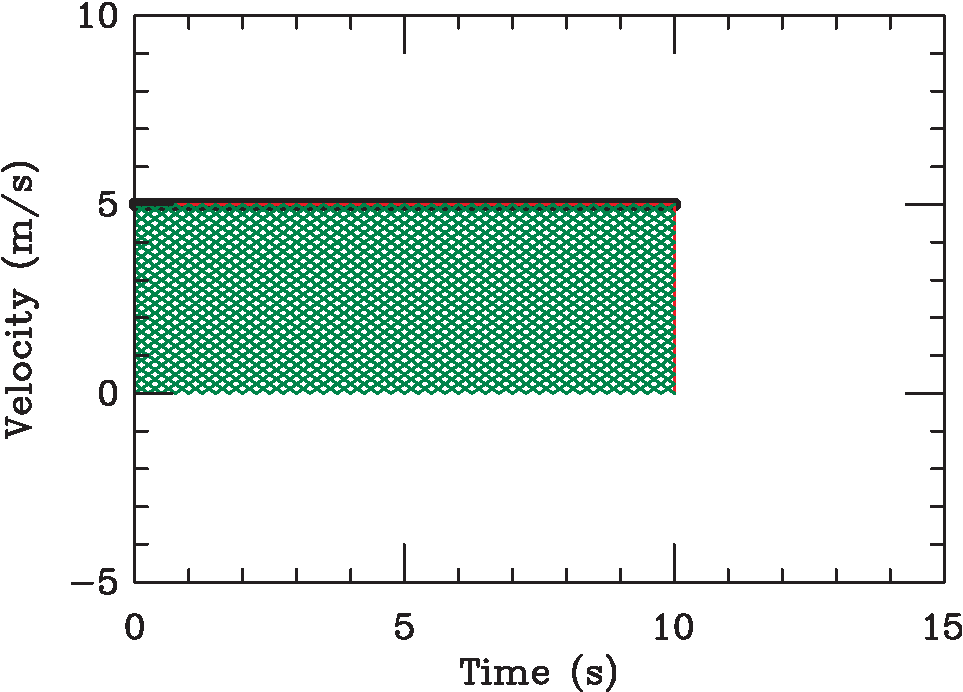
\includegraphics[width=0.7\textwidth]{integral-constant-crop.pdf}}

\bigskip
\bigskip

\centerline{\large We know $\Delta s = vt$. What is that here? What's the area of the shaded region?}

}


\frame{\frametitle{\textbf{A calculus review}}

\centerline{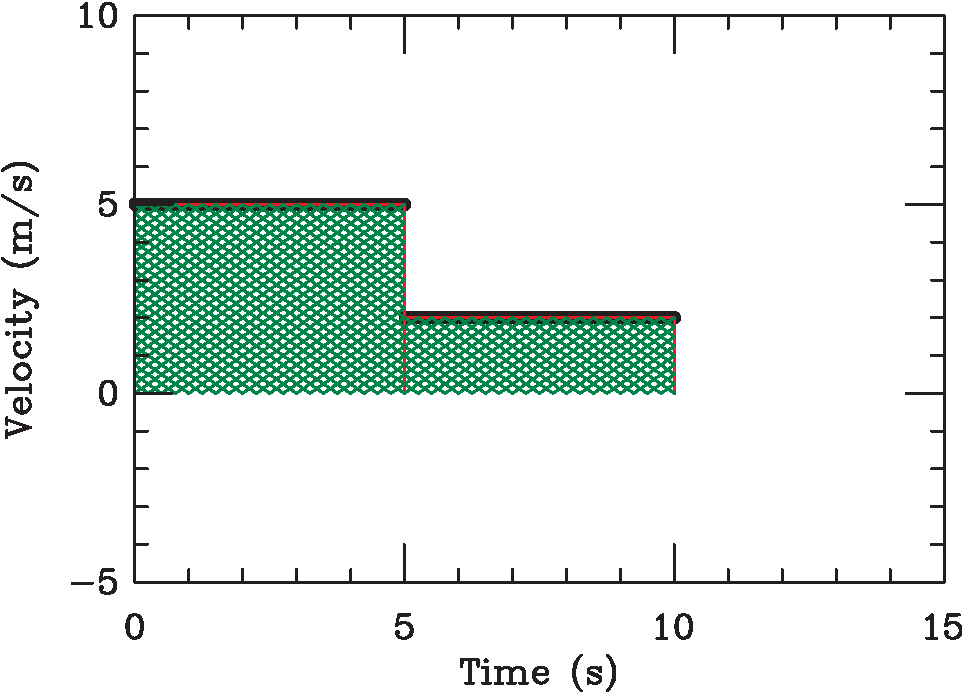
\includegraphics[width=0.6\textwidth]{integral-two-crop.pdf}}

\bigskip
\bigskip
\bigskip

\centerline{\large Now what is $\Delta s$? What is the area of the shaded region?}

}


\frame{\frametitle{\textbf{A calculus review}}

\centerline{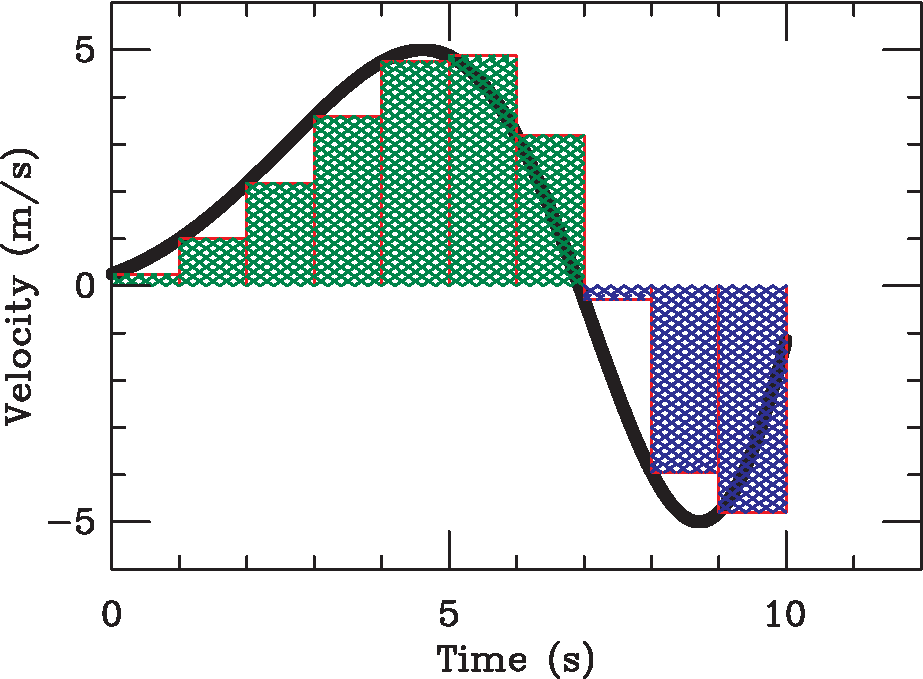
\includegraphics[width=0.6\textwidth]{integral-curve-coarse-crop.pdf}}

\bigskip
\bigskip
\bigskip

\centerline{\large Does this work? How do we fix it?}

}



\frame{\frametitle{\textbf{A calculus review}}

\centerline{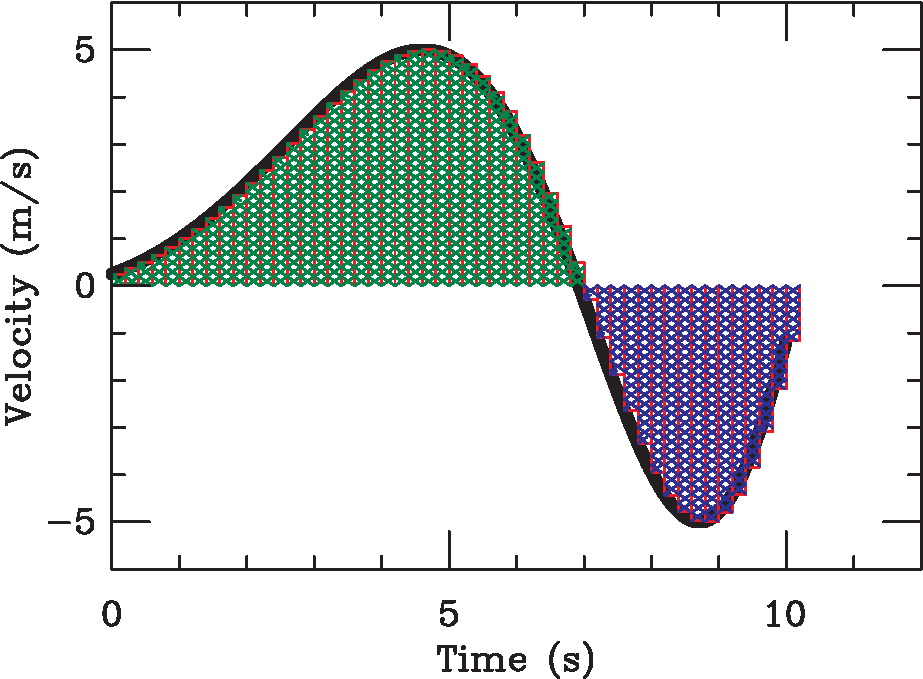
\includegraphics[width=0.6\textwidth]{integral-curve-fine-crop.pdf}}

\bigskip
\bigskip

\centerline{\large The area between the $t$-axis and the velocity curve is the distance traveled.}
\centerline{\large \color{Grey} (The area below the $t$-axis counts negative: ``the thing is going backwards''}
\bigskip
\centerline{\large In calculus notation: $\int v(t)\, dt = \delta s = s(t) - s_0$}

}

\frame{\frametitle{\textbf{Position, velocity, and acceleration}}
\begin{columns}
\column{0.125\textwidth}
\centerline{\Large Position}
\column{0.2\textwidth}
\small
{\color{Red}
\centerline{(derivative of)}
\centerline{rate of change of}
\centerline{$\xleftarrow{\makebox[\textwidth]{}}$}}
{\color{Green}
\color{Green}\centerline{$\xrightarrow{\makebox[\textwidth]{}}$}}
\color{Green}\centerline{area under the curve of}
\color{Green}\centerline{(integral of)}
\column{0.125\textwidth}
\centerline{\Large Velocity}
\pause
\column{0.2\textwidth}
\small
{\color{Red}
\centerline{(derivative of)}
\centerline{rate of change of}
\centerline{$\xleftarrow{\makebox[\textwidth]{}}$}}
{\color{Green}
\color{Green}\centerline{$\xrightarrow{\makebox[\textwidth]{}}$}}
\color{Green}\centerline{area under the curve of}
\color{Green}\centerline{(integral of)}
\column{0.15\textwidth}
\centerline{\Large Acceleration}
\end{columns}
}

\frame{\frametitle{\textbf{Constant acceleration}}
Particularly interesting situation: 
\BI
\item{Free fall (as you saw)}
\item{Any time the force is constant: $F = ma \rightarrow a = F/m$...}
\EI
\bigskip
\pause
Plan of attack:
\BI
\item{We know what the acceleration curve looks like (it's just flat)}
\item{Figure out the area under the acceleration curve to get the velocity curve}
\item{Figure out the area under the velocity curve to get the position curve}
\EI
\pause
\bigskip
\bigskip
\bigskip
\bigskip
Remember the area under the curve of (velocity, acceleration) just gives the {\it change in} (position, velocity) -- \ie initial minus final.

\bigskip
\bigskip

We'll start by assuming $s_0$ and $v_0$ are zero.
}

\frame{\frametitle{\textbf{Constant acceleration}}
\centerline{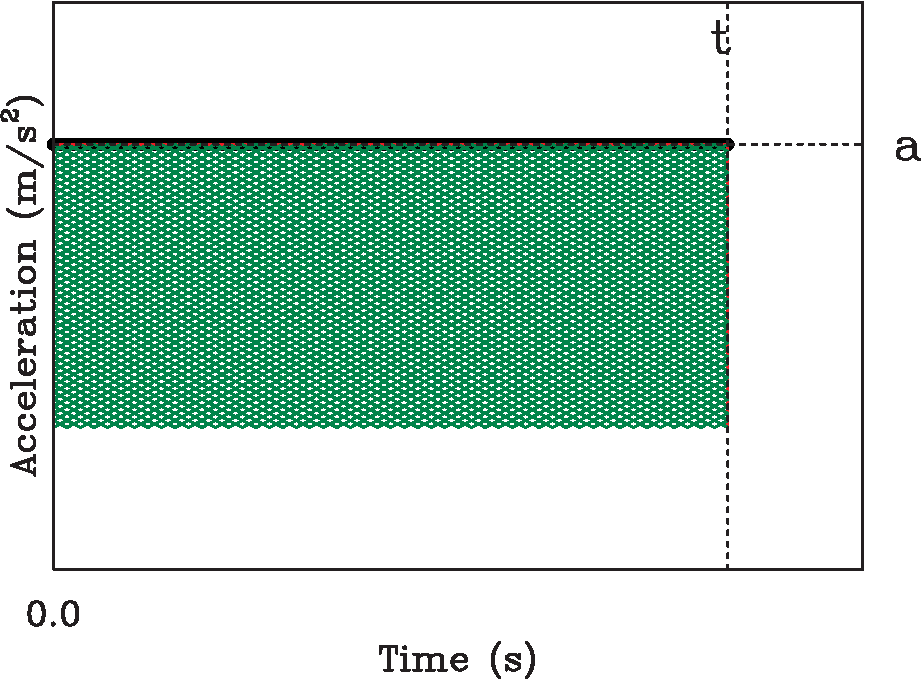
\includegraphics[width=0.6\textwidth]{area-under-a-crop.pdf}}

\bigskip
\bigskip

What's the area under the curve out to time $t$, which gives the change in the velocity -- $\Delta v=v(t) - v_0$?

\pause

\bigskip
\bigskip

\centerline{\Large $v(t) - v_0 = at$, so {\color{Red}$v(t) = at + v_0$}}
}


\frame{\frametitle{\textbf{Same thing again to get position}}
\centerline{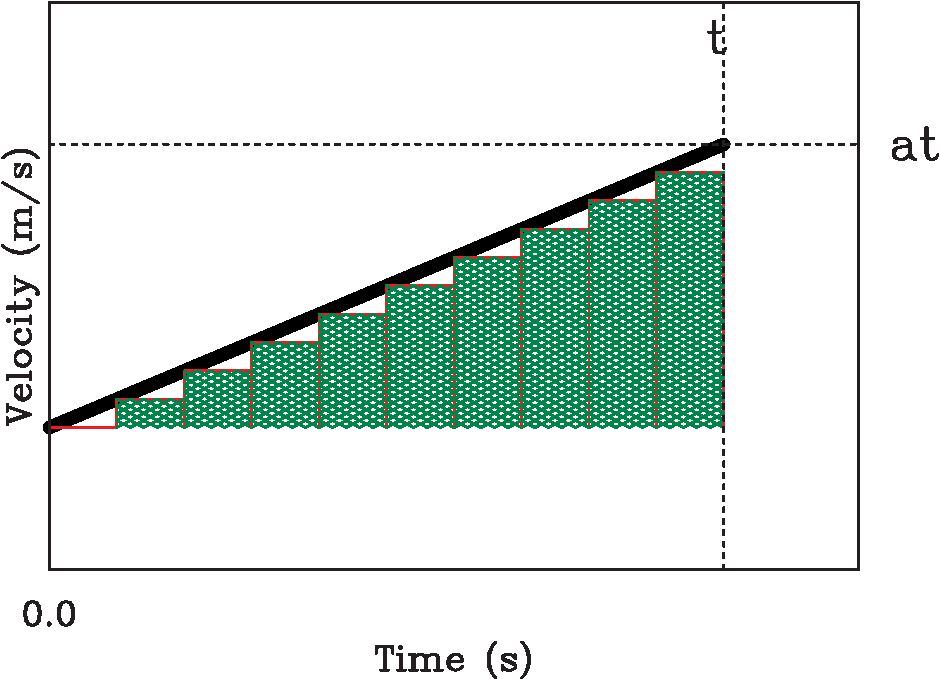
\includegraphics[width=0.6\textwidth]{area-under-v-crop.pdf}}

\bigskip
\bigskip

Now the area under the velocity curve gives the change in position: $\Delta s=s(t) - s_0$?

\pause

\bigskip
\bigskip

\centerline{\Large $s(t) - s_0 = \frac{1}{2}at^2$, thus $s(t) = \frac{1}{2}at + s_0$}
}

\frame{\frametitle{\textbf{Now if $v_0$ is not zero...}}
\centerline{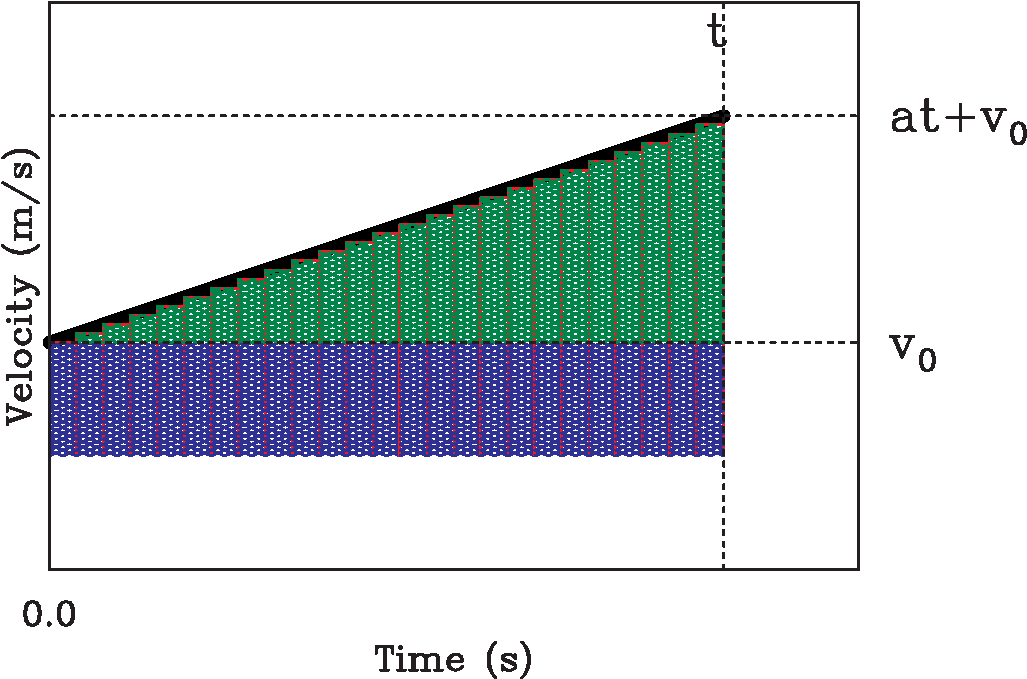
\includegraphics[width=0.6\textwidth]{area-under-v-full-crop.pdf}}

\bigskip

\pause
Area under blue part: $v_0 t$\\
Area under green part: $\frac{1}{2} at^2$\\
Total change in position: $s(t) - s_0 = \frac{1}{2}at^2 + v_0 t$

\bigskip
\bigskip
\centerline{\Large Thus, {\color{Red}$s(t) = \frac{1}{2}at^2 + v_0 t + s_0$}}
}

\frame{\frametitle{\textbf{For those who are familiar with calculus:}}

\begin{align*}
a(t) &= \rm{const}.\\
v(t) &= \int a\,dt &=& at + C_1 \\
s(t) &= \int v\,dt = \int (at + C_1) dt &=& \frac{1}{2}at^2 + C_1 t + C_2
\end{align*}

A little thought reveals that $C_1$ is the initial velocity $v_0$ and $C_2$ is the initial position $s_0$.\\
This gives us the things we just derived, but much more easily:


{\color{Red}
\Large
\begin{align*}
v(t) &=& at + v_0 \\
s(t) &=& \frac{1}{2}at^2 + v_0 t + s_0
\end{align*}}


}

\frame{\frametitle{\textbf{Example problems}}
\Large
\BI
\item{How long does it take for a falling object to fall 10 m?}
\EI
}

\frame{\frametitle{\textbf{Example problems}}
\Large
\BI
\item{You throw an object up with an initial speed of $5 m/s$. How high does it go? How long does it take to come back down?}
\EI
}




\end{document}

